\documentclass[11pt,a4paper]{article}
\usepackage[margin=1in]{geometry}
\usepackage{graphicx}
\usepackage{booktabs}
\usepackage{tabularx}
\usepackage{longtable}
\usepackage{array}
\usepackage{hyperref}
\usepackage{float}
\usepackage{caption}
\usepackage{xcolor}
\usepackage{enumitem}
\usepackage{microtype}
\usepackage{url}
\setlist{nosep}
\hypersetup{colorlinks=true,linkcolor=black,urlcolor=blue,citecolor=black}
\newcolumntype{Y}{>{\raggedright\arraybackslash}X}
\title{From BOAMP Notices to Procurement-Recurrence Risk:\\A Proxy-Event and Survival-Analysis Framework for Gigalis}
\author{First draft synthesis report}
\date{Generated from executed project outputs on 2026-07-08}

\begin{document}
\maketitle
\begin{abstract}
This synthesis turns the BOAMP analysis into one coherent argument for Gigalis. It separates the business question, the absence of official renewal-chain labels, the construction of a proxy recurrence event, the benchmark and diagnostic validation layers, the M0/M1/M2 method comparison, and the survival outputs used for 12- and 24-month operational prioritization. All reported values are traced in \texttt{source\_values\_used.csv}.
\end{abstract}
\tableofcontents
\clearpage

\section{Executive Summary}
Gigalis wants to anticipate future public digital procurement needs early enough to prepare account monitoring, segment planning, and commercial responses. BOAMP is useful for this objective because it records public notices over time, but it is not a contract-history database and it does not contain an official field linking an older call for tender to a later renewal.

The current selected event definition is \textbf{M2 balanced} with match-probability threshold 0.65. The final selected survival input is the M2 balanced survival CSV listed in the trace file. It contains 1,210 eligible contracts, 254 proxy recurrence events, and 956 censored rows, giving an event rate of 21.0\%. The event is an identifiable reappearance of a similar procurement need; it is not a verified legal renewal.

The selected M2 balanced method is benchmark-preferred over M0 balanced: benchmark-estimated precision/recall/F1 are 0.612/0.733/0.667, compared with 0.575/0.568/0.572 for M0 balanced. M0 balanced remains the conservative transparent baseline with 269 events and 22.2\%. The old 665-event result is historical pre-calibration only.

Under M2 balanced, the Kaplan-Meier median is not reached because fewer than half of contracts experience the selected proxy event before censoring. Estimated survival is 95.6\% at 12 months, 92.1\% at 24 months, 84.0\% at 48 months, and 76.0\% at 60 months. The reduced Cox C-index is 0.553; the richer category-aware Cox specification has C-index 0.606. LogNormalAFT is the best AFT model in the method-comparison output, with AIC 3357.9. Operational indicators are available for 1,204 contracts; median p12 is 0.0206, median p24 is 0.0634, and expected proxy recurrences are 29.0 at 12 months and 84.1 at 24 months.

\section{Internship and Business Context}
The internship project supports Gigalis in moving from retrospective procurement observation to forward-looking monitoring. The practical question is not only whether a buyer has purchased digital services before, but when a similar need may reappear and which buyers, segments, or contracts deserve attention during the next 12 to 24 months.

The output is therefore designed as a prioritization layer. It can help analysts and account managers decide where to monitor BOAMP publications, where to prepare domain expertise, and which digital segments may require earlier commercial preparation. The result should not be read as a deterministic renewal forecast. It is a structured risk indicator for observable BOAMP proxy recurrences.

\section{Data Source and Analytical Population}
BOAMP notices provide the public procurement corpus. The survival unit is the \texttt{APPEL\_OFFRE} notice because it represents the initial procurement opportunity whose later recurrence is being monitored. \texttt{ATTRIBUTION} notices are not treated as separate survival units; they are used for start-date refinement where available because award information can improve the timing of the original contract.

The current processed BOAMP file covers publication dates from 2015-03-02 to 2024-12-29. For the selected survival input, start dates run from 2015-03-02 to 2024-03-22. Rows are eligible when they have enough duration and timing information to define an observation window and either a selected proxy event or right-censoring.

\begin{table}[H]
\centering
\caption{Analytical population funnel. Source: executed BOAMP processed and selected M2 survival outputs.}

\begin{tabular}{lrrl}
\toprule
Step & Count & Share of previous & Source \\
\midrule
Raw BOAMP notices & 3,181 & -- & boamp\_full\_clean.csv \\
APPEL\_OFFRE notices & 1,933 & 60.8\% & boamp\_full\_clean.csv \\
Eligible contracts & 1,210 & 62.6\% & M2 survival input \\
Selected M2 proxy events & 254 & 21.0\% & M2 survival input \\
Censored rows & 956 & 79.0\% & M2 survival input \\
\bottomrule
\end{tabular}

\end{table}

\begin{figure}[H]
\centering
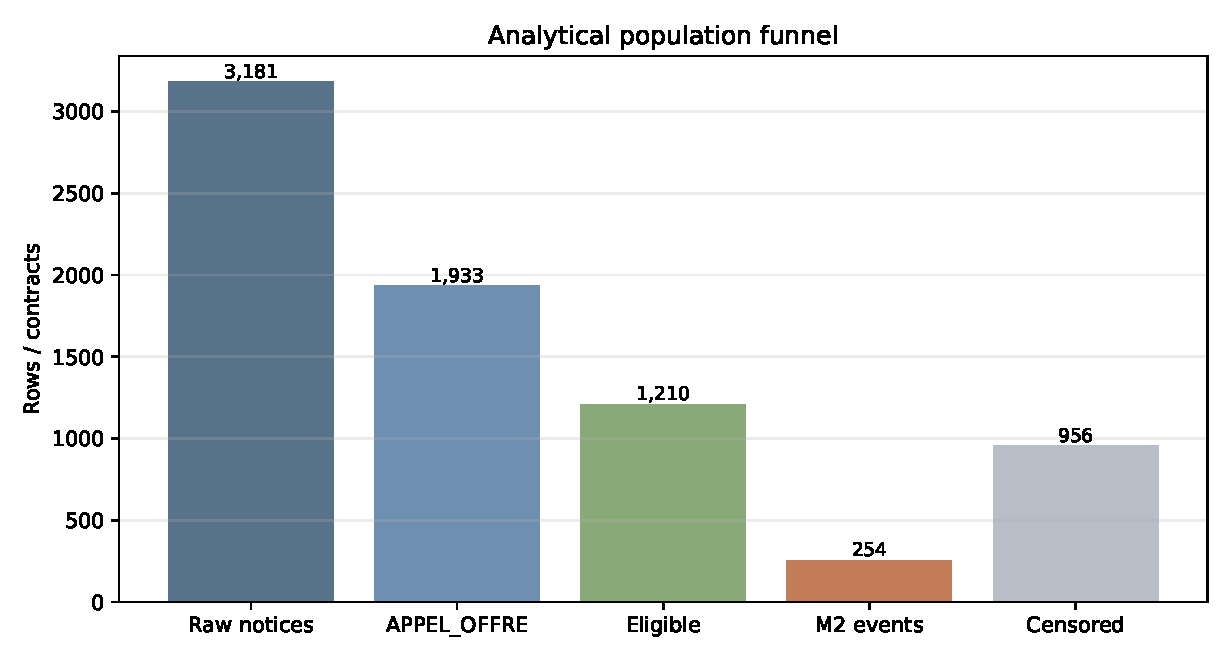
\includegraphics[width=.82\linewidth]{figures/fig_dataset_funnel.pdf}
\caption{Dataset funnel based on real BOAMP outputs. Source: generated from the executed project pipeline and validation outputs.}
\end{figure}

\section{Core Methodological Challenge: No Ground Truth}
BOAMP has no official renewal-chain ground truth. There is no field that reliably says one call for tender is the renewal of another, and real BOAMP precision and recall are therefore not directly observable. This matters because a later notice from the same buyer may be a genuine reappearance of a similar need, a related but different procurement, a publication artefact, or an unrelated requirement.

In this report, \textbf{event = 1} means a proxy recurrence under the selected rule: an identifiable reappearance of a similar procurement need. \textbf{event = 0} means censored or no observed proxy recurrence under the available data and rule. Neither label is legal ground truth. The validation vocabulary is therefore deliberately conservative: benchmark-estimated precision/recall, diagnostic evidence, negative-control diagnostics, and method-neutral review.

\section{Data Cleaning and Feature Construction}
The pipeline converts notice-level BOAMP data into a contract-level survival dataset. Buyer keys are constructed from available organization identifiers and cleaned buyer names; SIREN/SIRET enrichment helps reduce buyer fragmentation but does not eliminate it. CPV codes are normalized into division and category features, and generic CPV codes are flagged because broad codes such as software or IT services can create ambiguous links.

Duration cleaning preserves the raw duration when possible, flags suspicious values, and imputes administrative durations only when needed for survival construction. Start dates are built from publication dates and refined by attribution dates where available. Sentence-Transformer embeddings provide semantic similarity between source and candidate procurement objects. The technology taxonomy is provisional and based on CPV/keyword logic; supervised NLP classification is handled separately by the team and does not block the survival pipeline.

\section{Initial Baseline Method and Why It Was Replaced}
The initial baseline linked notices using semantic similarity, buyer agreement, CPV evidence, and timing around the expected end date. It produced 665 events among 1,210 eligible contracts, an event rate of 55.0\%. This high-linkage result was useful for exploration, but it maximized link quantity rather than analytical reliability.

Manual audit evidence showed low precision in parts of that baseline. Later analysis also showed that the manual audit sample was itself baseline-biased because it was stratified on the pre-calibration baseline's own links and confidence tiers. The project therefore changed objective: instead of maximizing the number of links, it constructs a calibrated proxy-event definition with transparent benchmark and diagnostic evidence. The 665-event result is retained only as a historical pre-calibration baseline.

\section{Synthetic BOAMP-like Benchmark}
The synthetic benchmark was needed because real BOAMP labels are unavailable. It creates BOAMP-like source and candidate pairs where the matching truth is known by construction. That makes it possible to estimate precision, recall, and F1 for candidate linkage rules without pretending that real BOAMP truth is observed.

The benchmark simulates buyer-name variation, generic CPV, CPV drift, missing CPV, missing duration, paraphrased text, timing shifts, and ambiguous same-buyer candidates. It uses easy, medium, and hard scenarios. The noise audit reports buyer-name-noise rates from 11.1% to 23.6%, generic-CPV rates from 8.6% to 15.4%, and missing-duration rates from 13.1% to 32.7% across scenarios.

\begin{table}[H]
\centering
\caption{Balanced-method synthetic benchmark performance by scenario, shown as precision/recall/F1. Source: synthetic benchmark outputs.}
\small
\begin{tabular}{lcccc}
\toprule
Method & Easy & Medium & Hard & Generic CPV \\
\midrule
M0 balanced & 0.777/0.806/0.791 & 0.601/0.586/0.593 & 0.318/0.302/0.310 & 0.464/0.525/0.493 \\
M1 balanced & 0.812/0.924/0.865 & 0.619/0.764/0.684 & 0.409/0.501/0.450 & 0.487/0.615/0.544 \\
M2 balanced & 0.812/0.924/0.865 & 0.619/0.764/0.684 & 0.409/0.501/0.450 & 0.487/0.615/0.544 \\
\bottomrule
\end{tabular}
\end{table}

\begin{figure}[H]
\centering
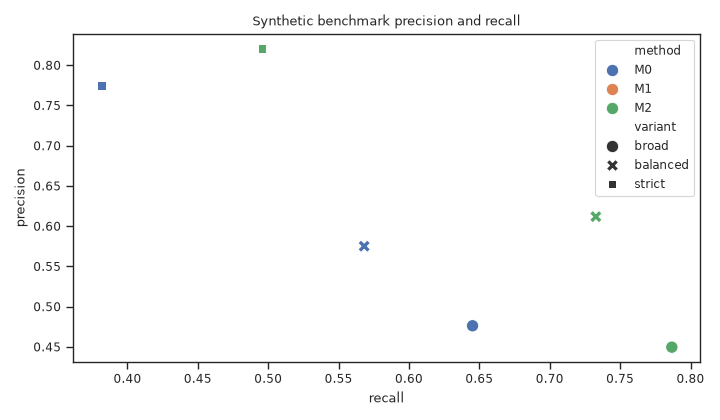
\includegraphics[width=.72\linewidth]{figures/fig_synthetic_precision_recall.png}
\caption{Synthetic precision-recall comparison for M0, M1, and M2. This is a controlled synthetic benchmark, not real BOAMP ground truth. Source: generated from the executed validation outputs.}
\end{figure}

\section{Linkage Method Comparison: M0, M1, M2}
M0 is the deterministic calibrated composite rule. It combines text similarity, CPV compatibility, timing, and buyer logic into transparent thresholds. M1 is a probabilistic linkage model trained on synthetic pair labels in the same feature space. M2 is an active-learning-assisted variant using the same probability feature space and producing a targeted review queue.

The current final recommendation promotes M2 balanced to the main method because all promotion criteria pass: the selection score is 0.797 versus 0.741 for M0 balanced; negative-control acceptance is lower than M0; the event count remains sufficient for survival; the synthetic-real profile shift is acceptable; and the text backend matches the real pipeline. Mapped audit precision is not used for final selection because the audit sample is baseline-biased. It remains a plausibility diagnostic only.

\begin{table}[H]
\centering
\caption{Method comparison. Synthetic metrics are benchmark-estimated; real event counts are proxy recurrences in BOAMP.}
\small
\resizebox{\linewidth}{!}{%
\begin{tabular}{lrrrrrrrl}
\toprule
Method & Prec. & Rec. & F1 & Events & Event rate & Neg. control & Cox C & Role \\
\midrule
M0 balanced & 0.575 & 0.568 & 0.572 & 269 & 22.2\% & 9.4\% & 0.544 & conservative baseline \\
M1 balanced & 0.612 & 0.733 & 0.667 & 256 & 21.2\% & 8.5\% & -- & alternative \\
M2 balanced & 0.612 & 0.733 & 0.667 & 254 & 21.0\% & 7.9\% & 0.553 & selected main \\
\bottomrule
\end{tabular}
}
\end{table}

\begin{figure}[H]
\centering
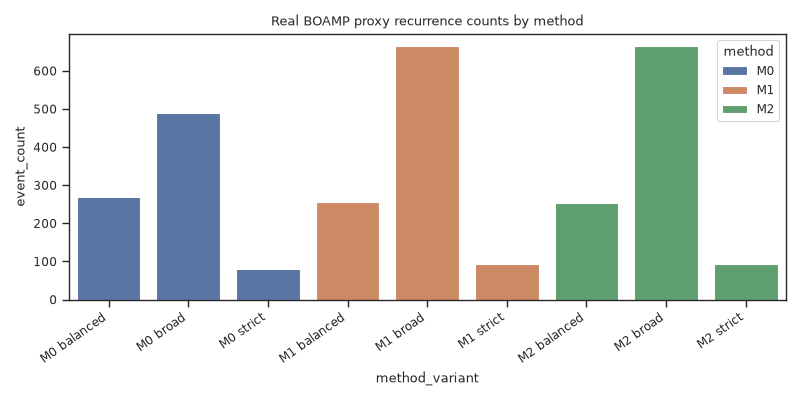
\includegraphics[width=.75\linewidth]{figures/fig_real_event_counts_by_method.png}
\caption{Real BOAMP proxy-event counts by method. Counts are constructed proxy events, not verified legal renewals. Source: generated from executed method-comparison outputs.}
\end{figure}

\section{Final Selected Event Definition}
The final selected definition is \textbf{M2 balanced}, a match-probability rule at threshold 0.65. The final dataset is \texttt{data/processed/boamp\_phase2\_survival\_method\_m2\_balanced.csv} with 1,210 eligible contracts, 254 events, 21.0\% event rate, and 956 censored rows.

M0 balanced remains the conservative transparent baseline: 269 events, 22.2\%, and negative-control acceptance 9.4\%. M0 strict is a high-confidence sensitivity with 79 events and 6.5\%. Broad rules are high-recall sensitivity checks. The old 665-event result is historical pre-calibration only.

\begin{figure}[H]
\centering
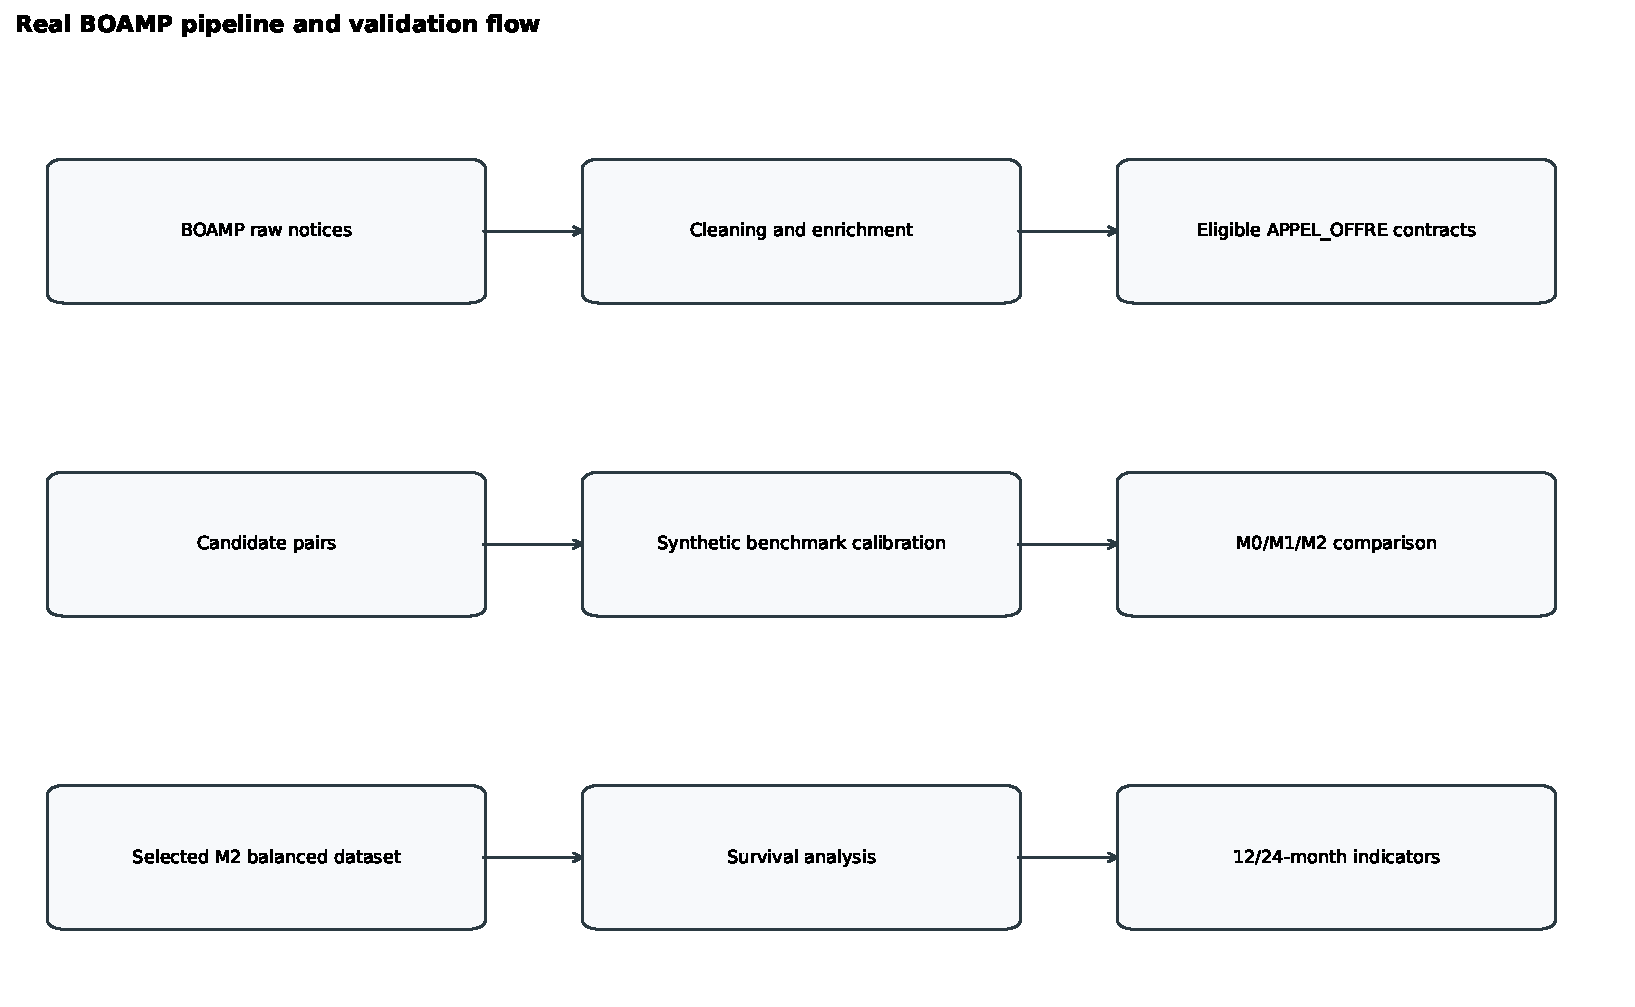
\includegraphics[width=.95\linewidth]{figures/fig_pipeline_overview.pdf}
\caption{Real BOAMP pipeline from raw notices to operational indicators. Source: generated from the executed project pipeline and validation outputs.}
\end{figure}

\section{Survival-Analysis Methodology}
The selected event definition creates a right-censored survival dataset. Each row has an observed duration: either the time from source start to the selected proxy recurrence, or the time from source start to censoring when no proxy recurrence is observed. Kaplan-Meier estimates the survival curve without assuming a parametric shape. Cox PH estimates relative hazard under proportional-hazard assumptions and reports C-index as a ranking-quality diagnostic. AFT models estimate parametric survival time distributions and are compared by AIC within the same event definition.

Fixed-horizon 12- and 24-month predictions translate the survival model into operational prioritization scores. These scores estimate identifiable BOAMP proxy recurrences under the model, not legal renewal probabilities. AIC values are comparable within the same event definition and specification; they should not be used to claim that one event definition is legally truer than another.

\begin{figure}[H]
\centering
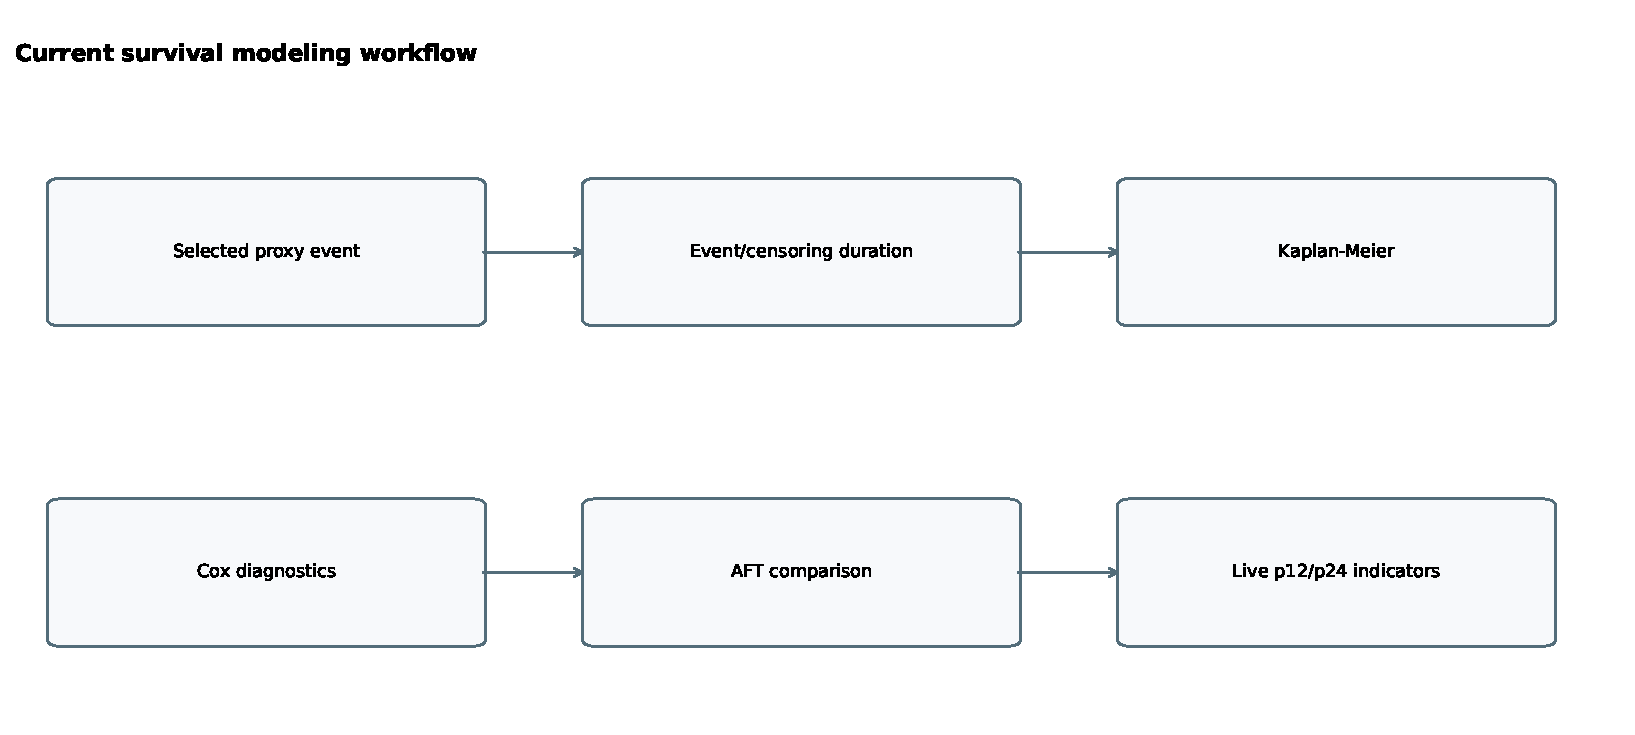
\includegraphics[width=.9\linewidth]{figures/fig_survival_modeling_workflow.pdf}
\caption{Survival modeling workflow for the selected M2 proxy-event definition. Source: generated from the executed project pipeline and validation outputs.}
\end{figure}

\section{Survival Results Under the Selected Method}
Under M2 balanced, there are 254 events among 1210 contracts. The Kaplan-Meier median is not reached because fewer than 50\% of contracts experience the selected proxy event before censoring. Survival is 95.6\% at 12 months, 92.1\% at 24 months, 84.0\% at 48 months, and 76.0\% at 60 months.

The reduced Cox C-index is 0.553; the richer category-aware specification reaches 0.606. PH diagnostics show a strong violation for declared duration (p = 3.59e-25), while imputation status (p = 0.728) and start year (p = 0.406) do not show the same violation. This supports using Cox mainly as a diagnostic ranking model and keeping AFT/fixed-horizon indicators central for operations.

The method-comparison output selects LogNormalAFT as the best AFT model with AIC 3357.9. The separate M2 AFT refit table also selects LogNormalAFT, with AIC 3360.5; this small difference is retained in \texttt{source\_values\_used.csv} because both values exist in executed outputs.

\begin{table}[H]
\centering
\caption{Survival headline comparison. Survival probabilities come from executed method-survival outputs.}
\small
\begin{tabular}{lrrrrrrr}
\toprule
Method & Events & KM median & S12 & S24 & S48 & S60 & Cox C \\
\midrule
M0 balanced & 269 & not reached & 95.9\% & 92.3\% & 83.2\% & 75.2\% & 0.544 \\
M2 balanced & 254 & not reached & 95.6\% & 92.1\% & 84.0\% & 76.0\% & 0.553 \\
M0 strict & 79 & not reached & 99.0\% & 98.1\% & 95.5\% & 91.6\% & 0.538 \\
\bottomrule
\end{tabular}
\end{table}

\begin{figure}[H]
\centering
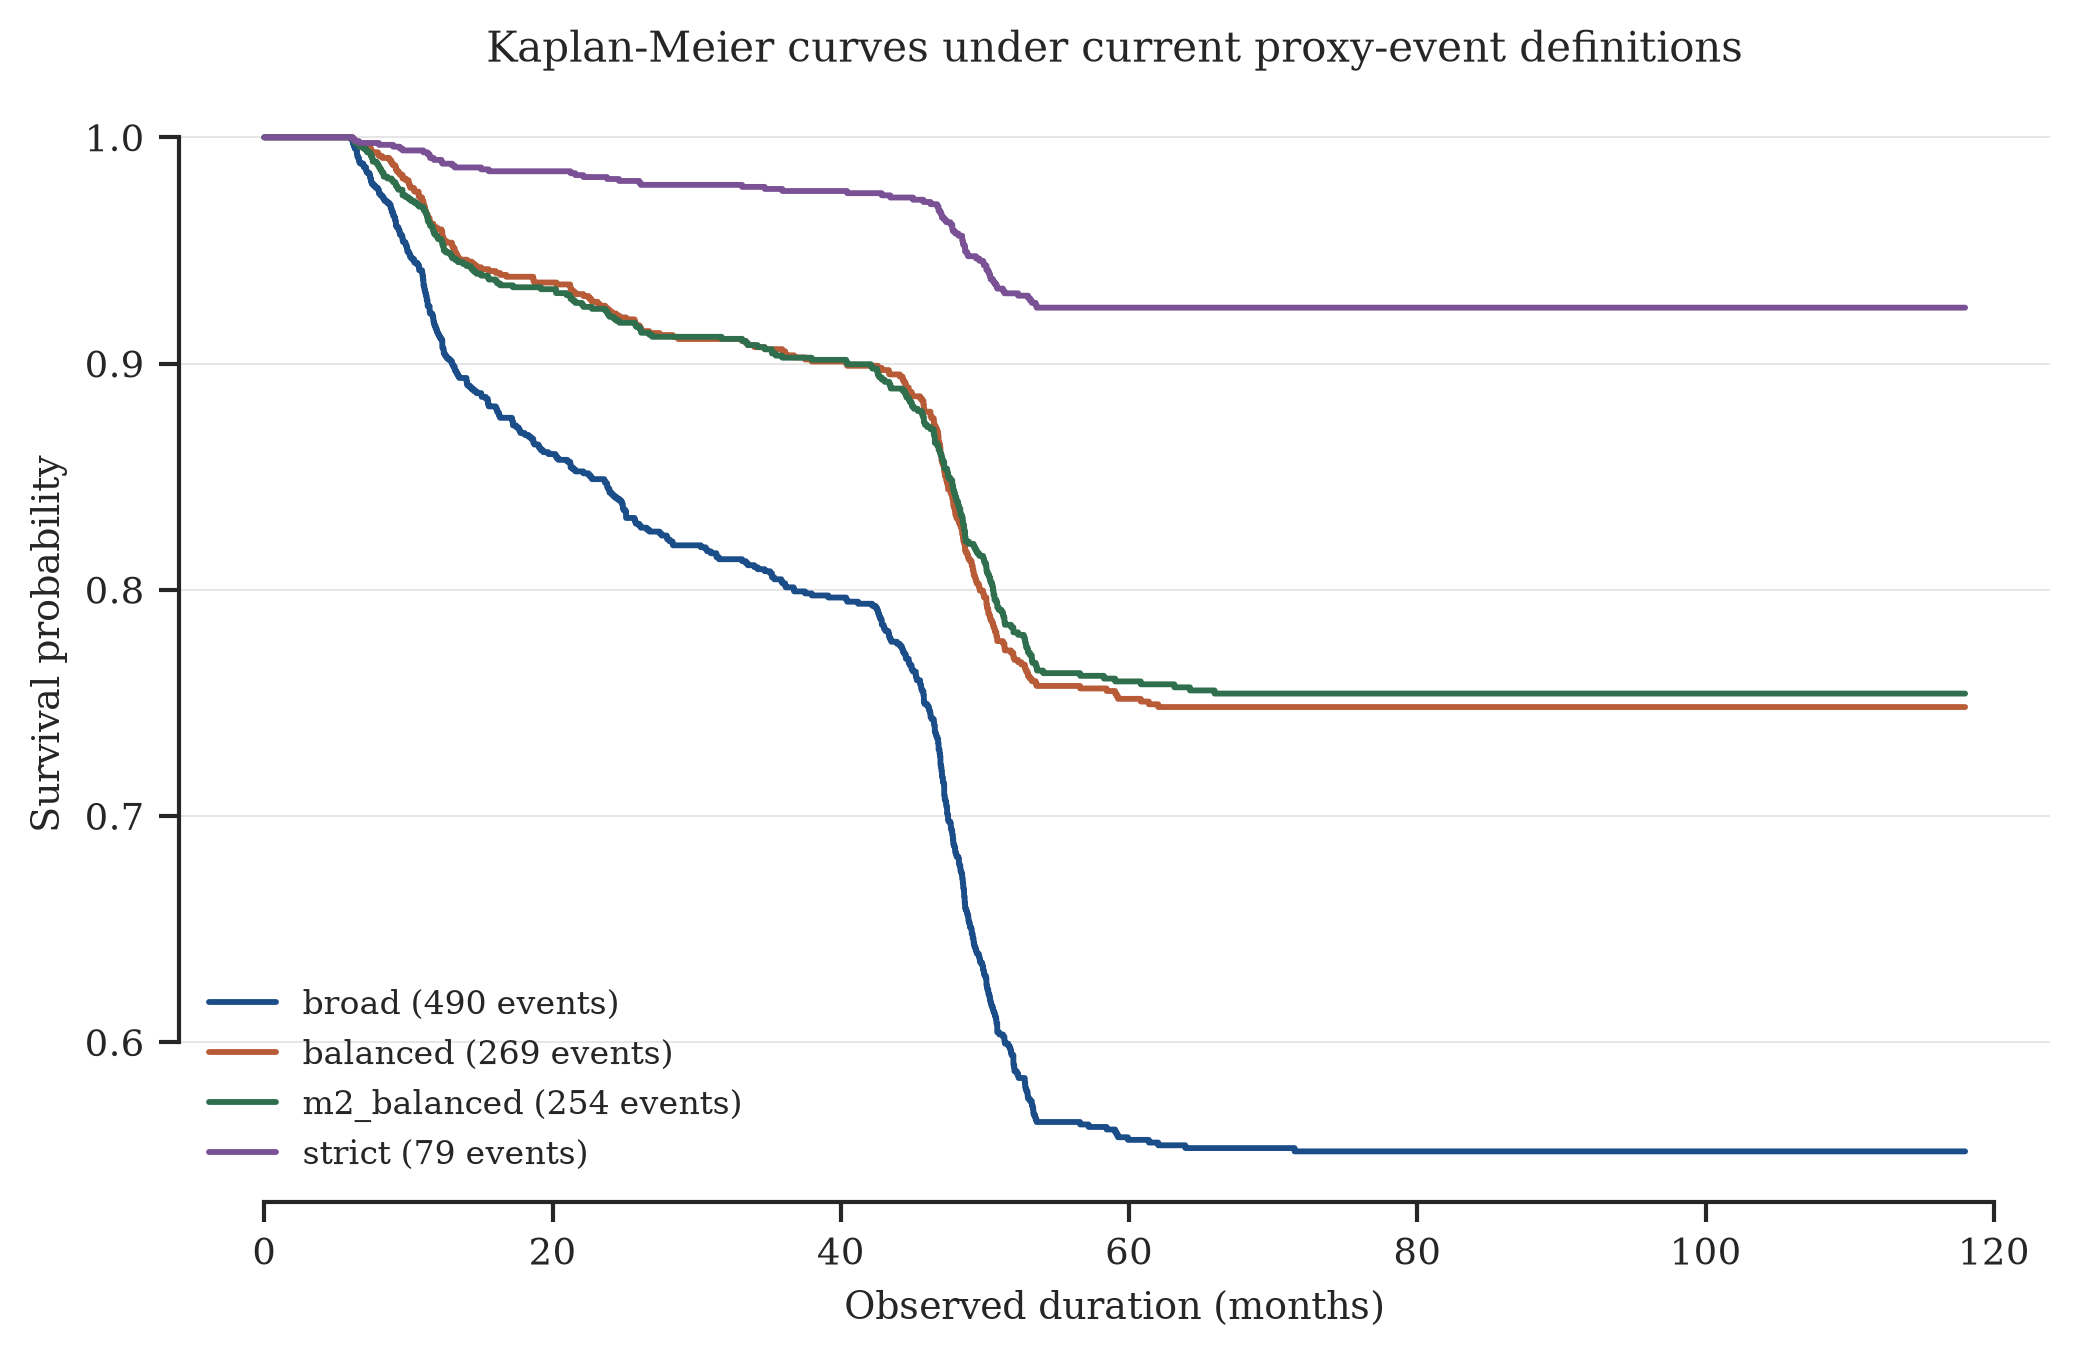
\includegraphics[width=.78\linewidth]{figures/fig_km_method_comparison.png}
\caption{Kaplan-Meier comparison for real BOAMP proxy-event definitions. Source: generated from executed survival outputs.}
\end{figure}

\section{Operational 12/24-Month Indicators}
The selected survival model is converted into contract-level p12 and p24 scores. These are prioritization scores for identifiable BOAMP proxy recurrences. They can support monitoring lists and segment planning, especially where many small probabilities aggregate into a meaningful buyer or segment workload.

Operational indicators are available for 1,204 contracts. The median 12-month score is 0.0206; the median 24-month score is 0.0634. Summed across scored contracts, expected proxy recurrences are 29.0 at 12 months and 84.1 at 24 months.

\begin{table}[H]
\centering
\caption{Top buyer-level expected proxy recurrences under M2 balanced. Source: survival model output.}
\small
\begin{tabular}{lrrr}
\toprule
Buyer key & Contracts & Expected 12m & Expected 24m \\
\midrule
SIREN:234400034 & 91 & 2.8 & 7.7 \\
NAME:nantes metropole & 72 & 1.6 & 4.7 \\
SIREN:935367433 & 28 & 1.0 & 2.7 \\
SIREN:264400136 & 42 & 0.9 & 2.6 \\
SIREN:391722881 & 28 & 0.9 & 2.4 \\
SIREN:244900015 & 30 & 0.7 & 2.0 \\
\bottomrule
\end{tabular}
\end{table}

\begin{table}[H]
\centering
\caption{Top segment-level expected proxy recurrences under M2 balanced. Source: survival model output.}
\small
\begin{tabular}{lrrr}
\toprule
Segment & Contracts & Expected 12m & Expected 24m \\
\midrule
IT Services \& Consulting & 343 & 11.9 & 32.4 \\
Software \& Applications & 223 & 3.7 & 11.6 \\
Cybersecurity & 136 & 3.4 & 9.8 \\
Telecom \& Networks & 220 & 3.3 & 10.4 \\
Unknown & 114 & 2.7 & 8.0 \\
Digital Workplace \& Collaboration & 51 & 1.2 & 3.5 \\
\bottomrule
\end{tabular}
\end{table}

\begin{figure}[H]
\centering
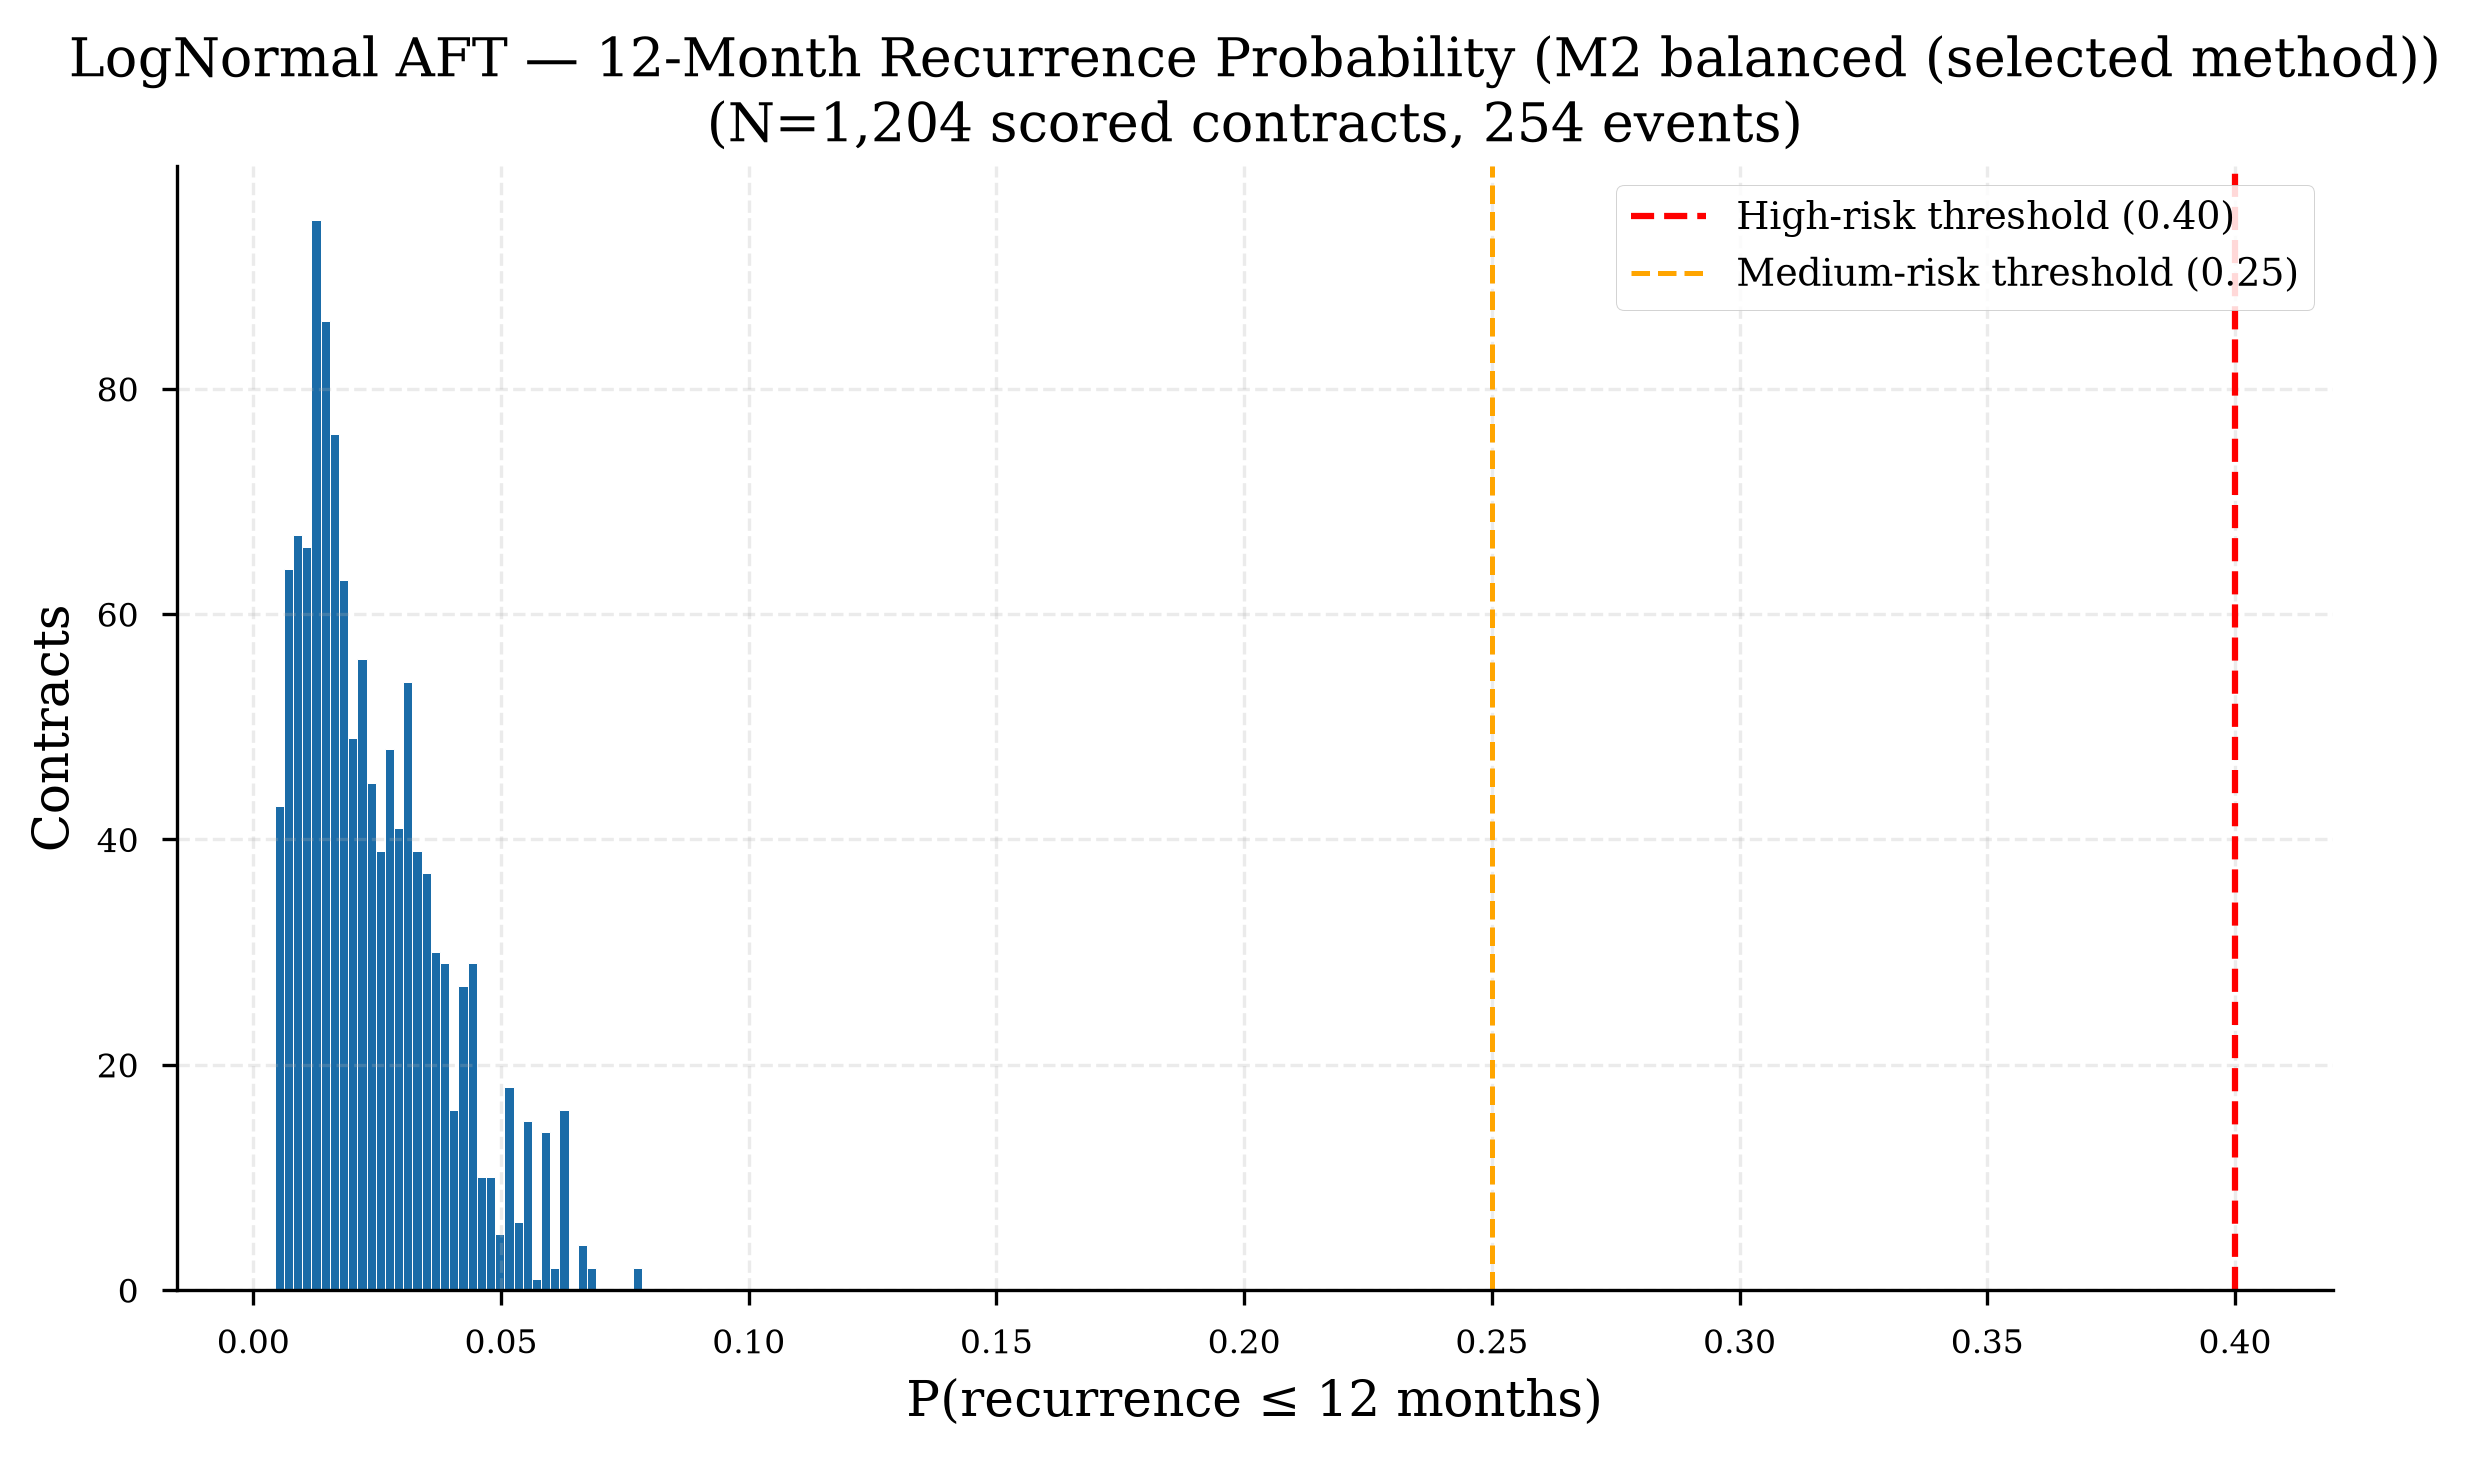
\includegraphics[width=.72\linewidth]{figures/fig_m2_risk_distribution.png}
\caption{Distribution of 12-month proxy-recurrence prioritization scores under M2 balanced. Source: survival model output.}
\end{figure}

\section{Robustness and Sensitivity}
The survival conclusions are stable across M0 balanced and M2 balanced in the current outputs. M0 balanced has 95.9\% 12-month survival and 92.3\% 24-month survival, while M2 balanced has 95.6\% and 92.1\%. This supports the applied interpretation that most contracts do not show an identifiable proxy recurrence within the first two years.

M0 strict is mainly a lower-bound sensitivity: it has only 79 events and 6.5\% event rate. Broad rules are useful to check high-recall behavior but are not selected for the main survival model. M2 has a higher generic-CPV share than M0 balanced (37.0\% versus 23.0\%), so generic-CPV M2 links should be reviewed first in the next manual validation pass.

\section{Limitations}
\begin{longtable}{p{.27\linewidth}p{.32\linewidth}p{.32\linewidth}}
\caption{Limitations and mitigations.}\\
\toprule
Limitation & Consequence & Mitigation / current status \\
\midrule
\endfirsthead
\toprule
Limitation & Consequence & Mitigation / current status \\
\midrule
\endhead

No real BOAMP ground truth & Real precision and recall cannot be observed directly & Report proxy recurrence only; use method-neutral review next \\
Synthetic benchmark is controlled, not real truth & Benchmark-estimated metrics may not transfer perfectly & Treat as calibration evidence, not proof \\
Manual audit baseline bias & Mapped audit precision is not a final arbiter & Use as plausibility diagnostic only \\
Active-learning review sample not completed & M2 review queue has not become validation labels & Complete method-neutral manual review \\
Generic CPV risk & Higher M2 generic-CPV share may hide weaker semantic evidence & Review generic-CPV M2 links first \\
Buyer fragmentation remains & Same organization can appear under multiple buyer keys & Continue SIREN/SIRET enrichment and matching checks \\
Declared duration is administrative and violates PH & Reduced Cox assumptions are partly strained & Prefer AFT and fixed-horizon indicators for operations \\
Cox C-index is weak-to-moderate & Ranking power is useful but limited & Present risk scores as prioritization, not certainty \\
Supervised NLP classifier handled separately & Segment labels are provisional in this survival work & Integrate final team NLP labels when available \\
Trend/change-point analysis remains future work & The report does not yet model demand shifts over calendar time & Add Phase 4 trend analysis later \\

\bottomrule
\end{longtable}

\section{Conclusion and Next Steps}
The project now has a calibrated, traceable proxy-event definition for BOAMP recurrence analysis. The selected main method is M2 balanced; M0 balanced remains the conservative transparent baseline; the old 665-event output is historical pre-calibration only. Survival analysis under the selected method produces readable 12- and 24-month indicators for operational prioritization.

The next work should focus on method-neutral manual review of M2 links, inspection of generic-CPV M2 links, integration of final NLP labels when the separate team classifier is available, Phase 4 trend/change-point analysis, and optional DECP enrichment. Those steps would make the operational layer more robust without changing the central interpretation: BOAMP does not provide legal renewal ground truth, so the analysis must remain explicit about proxy recurrence and diagnostic evidence.

\appendix
\clearpage
\section{Validation Framework Diagrams}
\begin{figure}[H]
\centering
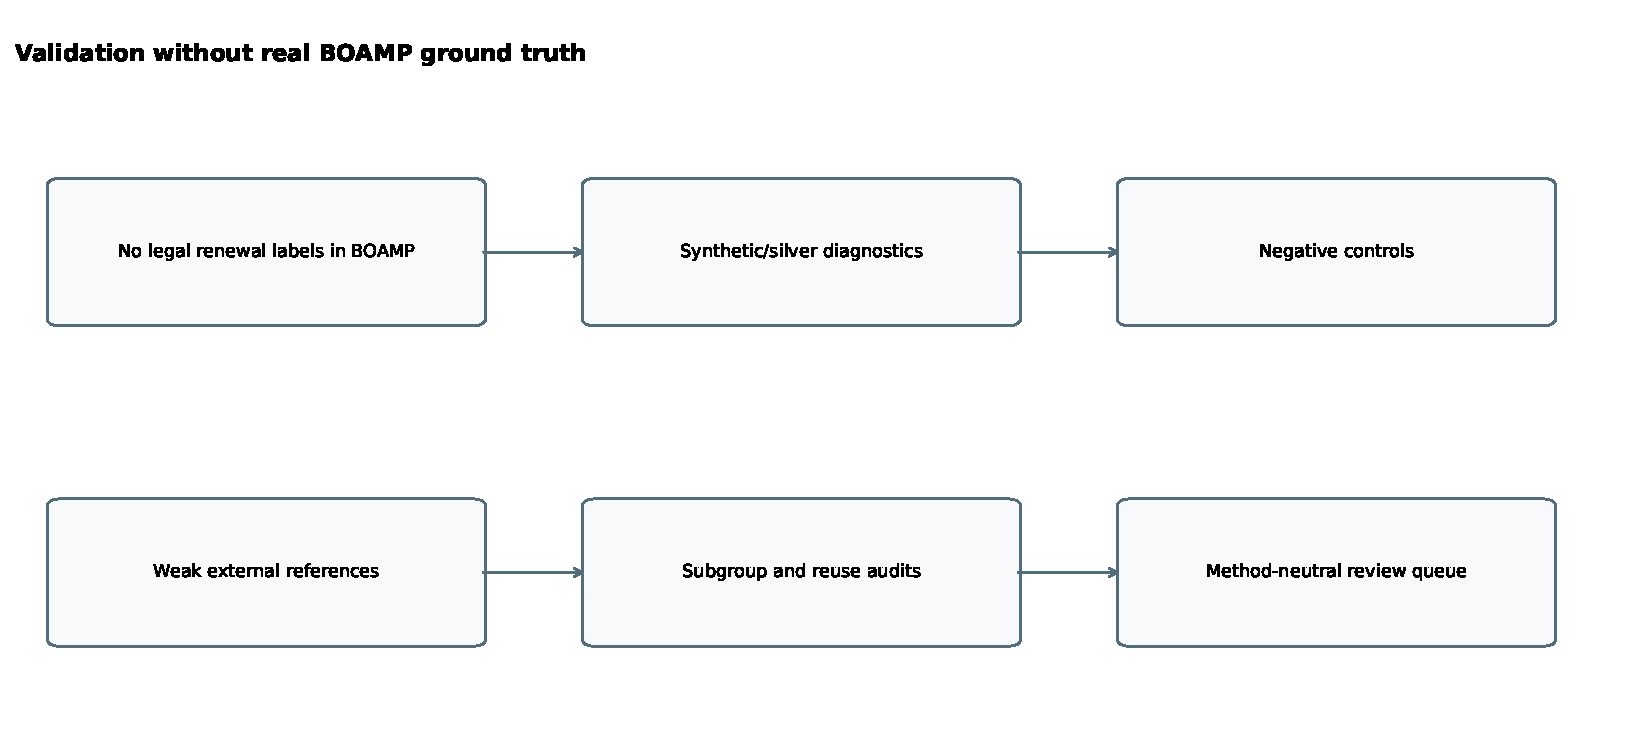
\includegraphics[width=.9\linewidth]{figures/fig_no_ground_truth_validation_framework.pdf}
\caption{Validation framework in a no-ground-truth BOAMP setting. Source: generated from the executed project pipeline and validation outputs.}
\end{figure}

\begin{figure}[H]
\centering
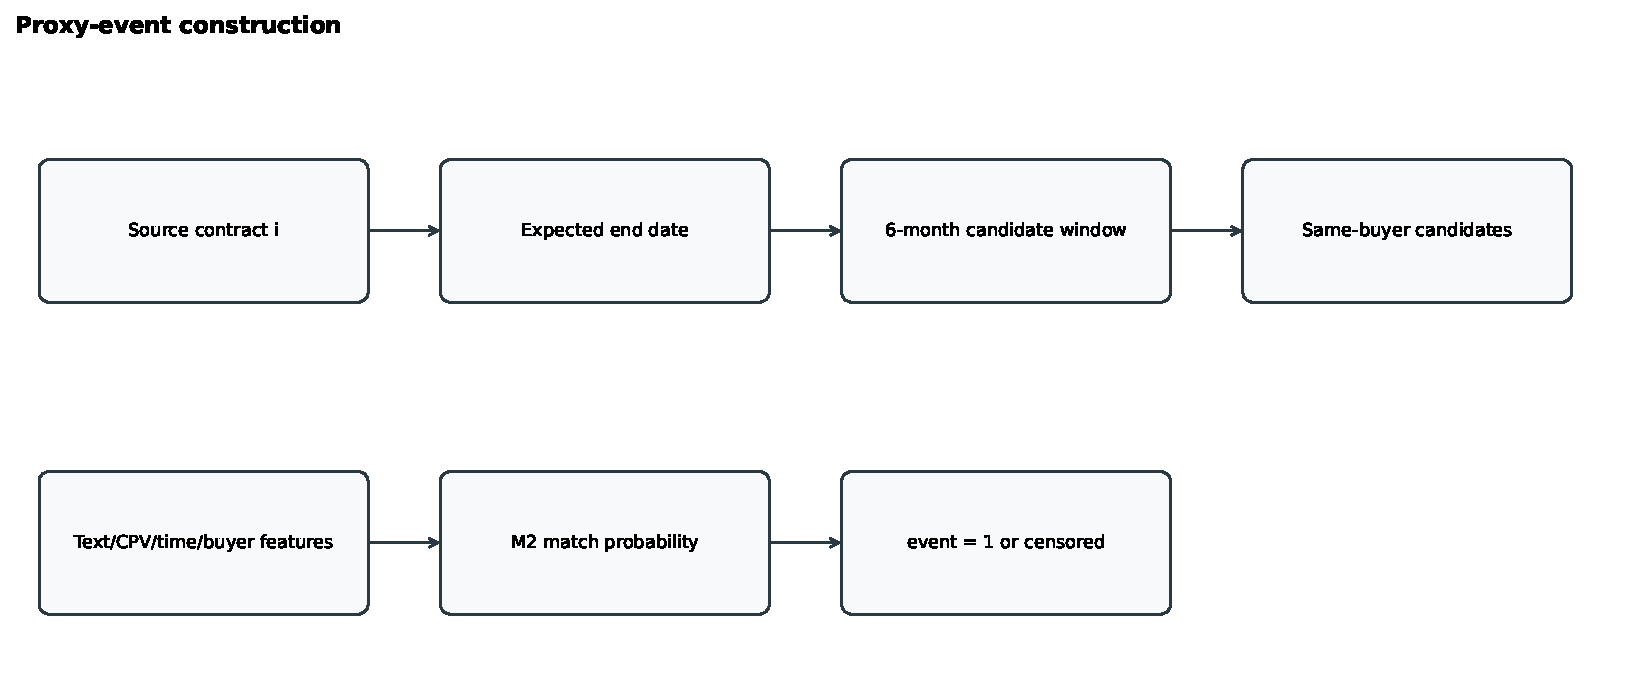
\includegraphics[width=.86\linewidth]{figures/fig_proxy_event_construction.pdf}
\caption{Proxy-event construction diagram for real BOAMP candidate links. Source: generated from the executed project pipeline and validation outputs.}
\end{figure}

\begin{figure}[H]
\centering
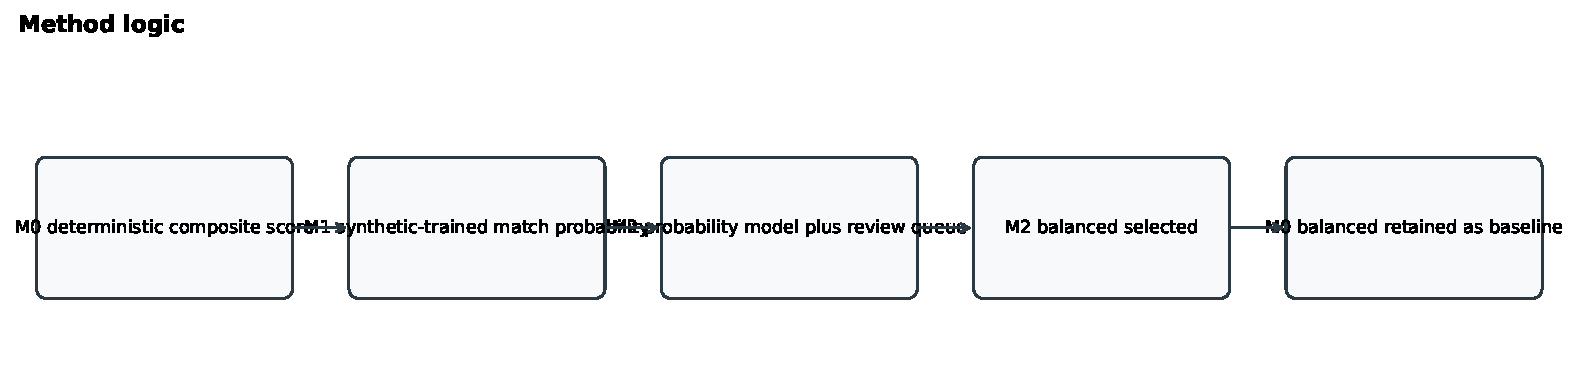
\includegraphics[width=.9\linewidth]{figures/fig_m0_m1_m2_method_logic.pdf}
\caption{M0/M1/M2 method logic. Source: generated from the executed project pipeline and validation outputs.}
\end{figure}

\section{Top Contract Indicators}
\begin{table}[H]
\centering
\caption{Top contract-level p12/p24 scores under M2 balanced. Source: survival model output.}
\small
\begin{tabular}{llrr}
\toprule
Contract & Segment & p12 & p24 \\
\midrule
BOAMP:24-12133 & IT Services \& Consulting & 0.0785 & 0.1839 \\
BOAMP:24-21999 & IT Services \& Consulting & 0.0777 & 0.1824 \\
BOAMP:22-112462 & IT Services \& Consulting & 0.0692 & 0.1665 \\
BOAMP:22-153148 & IT Services \& Consulting & 0.0677 & 0.1637 \\
BOAMP:22-123056 & IT Services \& Consulting & 0.0668 & 0.1621 \\
BOAMP:23-20260 & IT Services \& Consulting & 0.0668 & 0.1621 \\
BOAMP:23-41937 & IT Services \& Consulting & 0.0668 & 0.1621 \\
BOAMP:23-92003 & IT Services \& Consulting & 0.0668 & 0.1621 \\
\bottomrule
\end{tabular}
\end{table}

\begin{figure}[H]
\centering
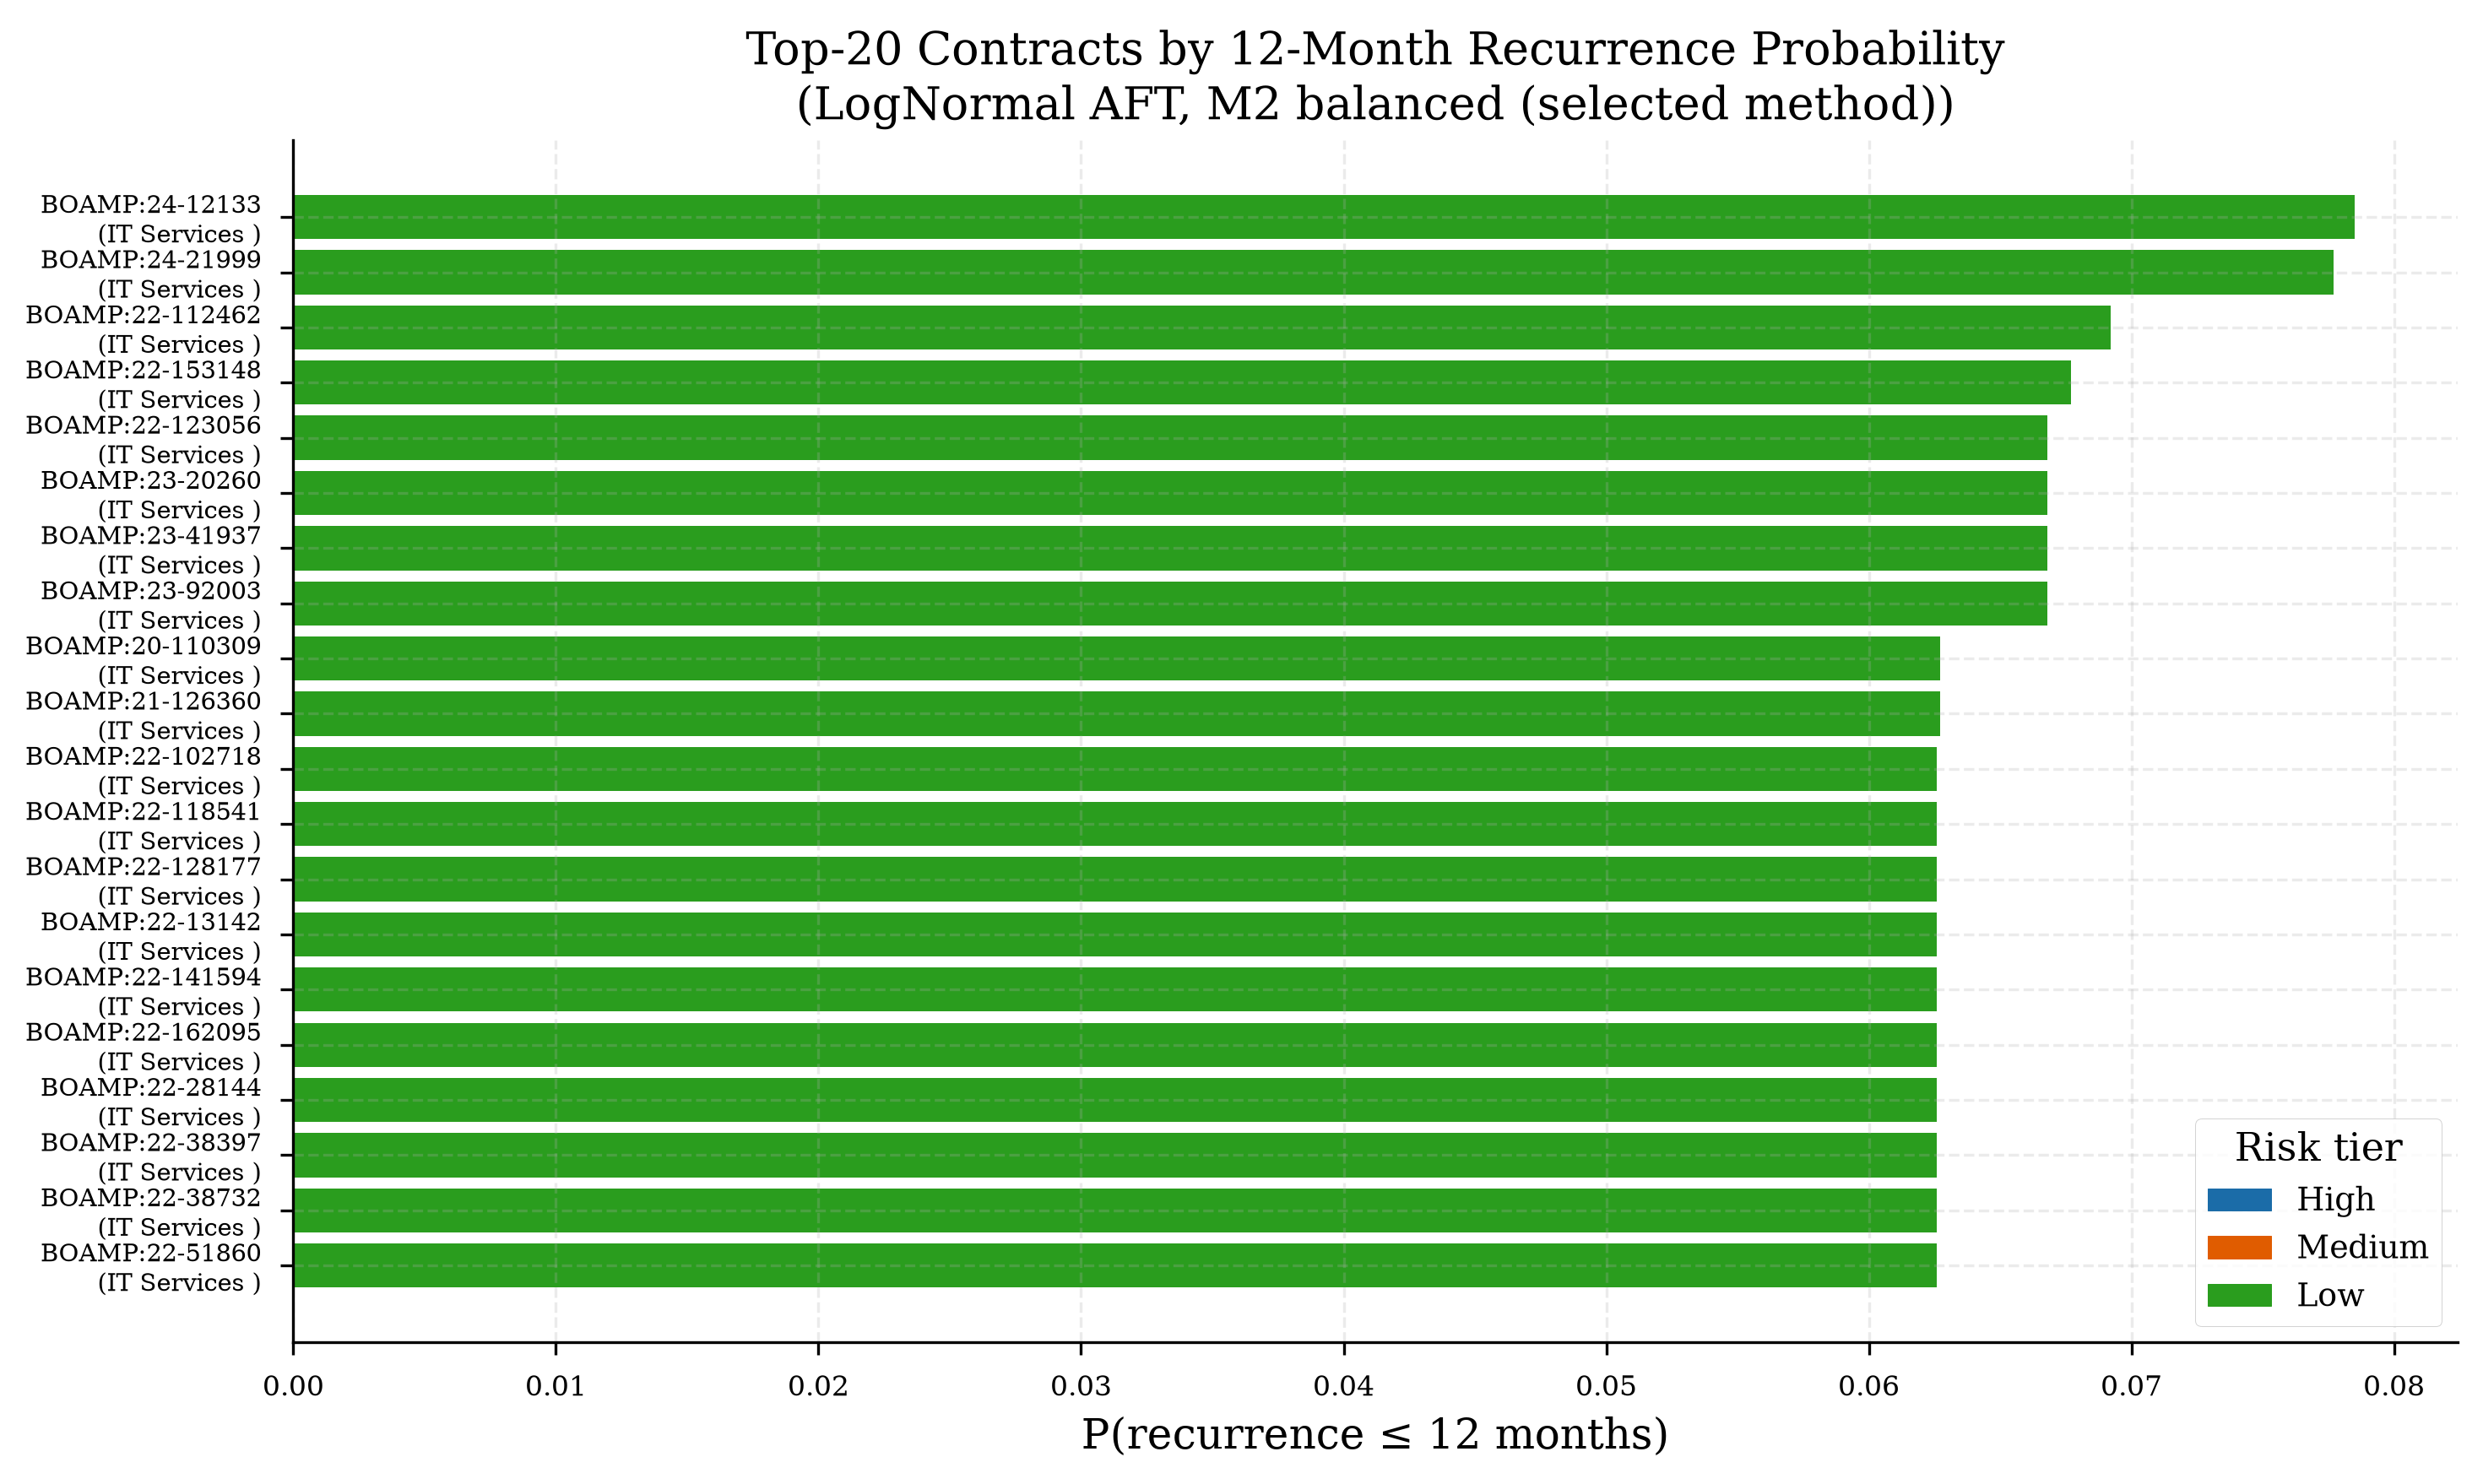
\includegraphics[width=.82\linewidth]{figures/fig_top_contracts_m2_balanced.png}
\caption{Top contract-level 12/24-month proxy-recurrence scores under M2 balanced. Source: survival model output.}
\end{figure}

\clearpage
\section{Source Trace Extract}
The complete trace table is stored in \texttt{source\_values\_used.csv}. The extract below shows the main headline values and their executed output sources.

\begin{longtable}{@{}p{.18\linewidth}p{.24\linewidth}p{.20\linewidth}p{.28\linewidth}@{}}
\caption{Extract from the source trace table.}\\
\toprule
Section & Metric & Value & Source file \\
\midrule
\endfirsthead
\toprule
Section & Metric & Value & Source file \\
\midrule
\endhead
selection & selected method & M2 balanced & final recommendation \\
selection & threshold & 0.65 & probabilistic linkage results \\
population & raw BOAMP notices & 3,181 & cleaned BOAMP data \\
population & APPEL\_OFFRE notices & 1,933 & cleaned BOAMP data \\
population & eligible contracts & 1,210 & M2 balanced survival input \\
population & selected M2 events & 254 & M2 balanced survival input \\
population & selected M2 censored rows & 956 & M2 balanced survival input \\
historical & pre-calibration events & 665 & historical handoff \\
method comparison & M2 synthetic precision/recall/F1 & 0.612 / 0.733 / 0.667 & synthetic metrics \\
method comparison & M2 negative-control acceptance & 7.9\% & method comparison \\
survival & M2 survival 12/24/48/60m & 95.6\% / 92.1\% / 84.0\% / 76.0\% & method survival comparison \\
survival & reduced Cox C-index & 0.553 & method survival comparison \\
survival & richer Cox C-index & 0.606 & category-aware Cox table \\
survival & best AFT / AIC & LogNormalAFT / 3357.9 & method survival comparison \\
operational & scored contracts & 1,204 & M2 risk indicators \\
operational & median p12 / p24 & 0.0206 / 0.0634 & M2 risk indicators \\
operational & expected 12/24m recurrences & 29.0 / 84.1 & M2 risk indicators \\
\bottomrule
\end{longtable}

\clearpage
\section{Internal References}
This first draft uses only existing project outputs and method names already present in the repository. The main internal sources are the final method recommendation table, the linkage method comparison tables, the method survival comparison table, the M2 balanced 12/24-month risk table, and the selected M2 balanced survival input. Exact paths are listed in \texttt{source\_values\_used.csv}. External literature citations can be added later if the report is expanded into a formal academic manuscript.

\end{document}
